\chapter{АППАРАТНАЯ ЧАСТЬ}
\section{Конструирование макета}
	По структурной схеме (рис. 2.7) создадим схему электрическую принципиальную. 
	
	\begin{figure}[H]
    \centering
    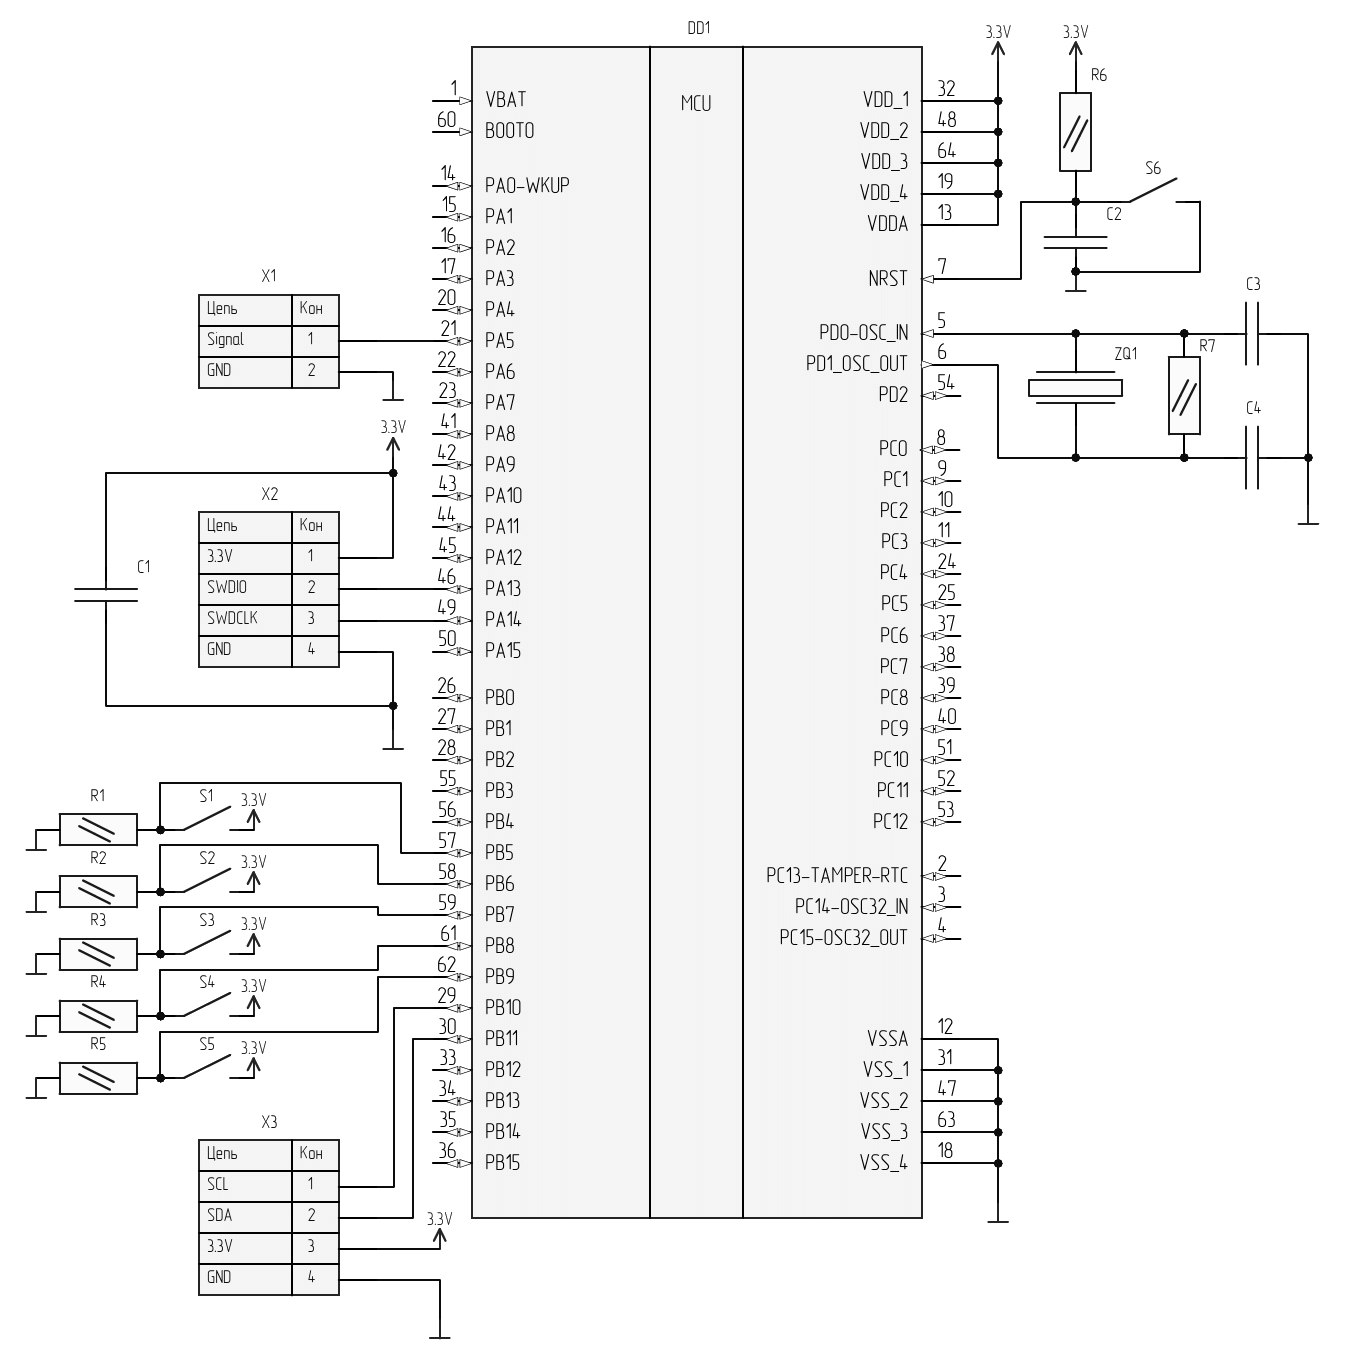
\includegraphics[width=1\textwidth]{../image/scheme-cropped.png}
    \caption{Схема электрическая принципиальная.}
	\end{figure}
	
	Просто так контроллер работать не сможет. Необходим внешний кварцевый резонатор для стабилизации частоты системного тактового генератора, а также функция сброса. Эти узлы уже реализованы на отладочной плате микроконтроллера. Питание схемы будет подаваться через разъём SWD.
	
	Для управления потребуется 5 кнопок
	\begin{enumerate}
		\item Уменьшить частоту.
		\item Увеличить частоту.
		\item Предыдущий сигнал.
		\item Следующий сигнал.
		\item Выбор шага.
	\end{enumerate}
	
	Выделим для кнопок выводы PB5 - PB9. Постоянно быть подключенными к напряжению или земле выводы не могут, т. к. не будет возможности подавать на них какой-либо информационный сигнал. На выводы могут наводиться произвольные потенциалы, что негативно влияет на работу схемы. Подобные потенциалы имитируют сигналы, которые не предусмотрены. Из-за них может нарушиться логика работы, поэтому их принято фиксировать~\cite{schemat}. 
	
	Для этого используют подтягивающие (Pull - up) или заземляющие (Pull - down) резисторы. Они создают цепь, которая обеспечивает подтяжку сигнала к напряжению питания или земле. Если резисторы имеют большие сопротивления, то сигналы относят к слабым. При подключении сильных информационных сигналов происходит преодоление слабых и функциональность схемы не нарушается~\cite{butres}.
	
	\begin{figure}[H]
    \centering
    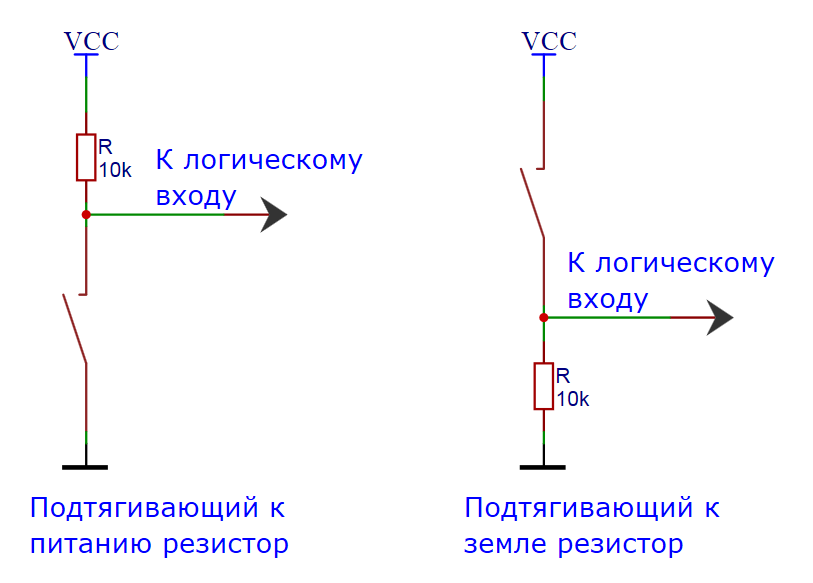
\includegraphics[width=0.55\textwidth]{../image/res.png}
    \caption{Pull-up и Pull - down резисторы.}
	\end{figure}
	
	В схеме устройства будет использоваться подтяжка к земле для считывания высокого уровня сигнала, то есть будет использоваться прямая логика. Рассчитаем минимальное и максимальное сопротивление заземляющего резистора.
	\begin{gather}
	R_{min} = \dfrac{V_{0}}{I_{max}},
	\end{gather}
	
	где $V_{0}$ --- напряжение логического нуля,
	
	$I_{max}$ --- максимальный ток вывода.
	
	Согласно спецификации микроконтроллера напряжение логического нуля составляет 1,16 В, а максимальный протекающий ток через пин может быть 25 мА~\cite{f103}. 
	
\begin{center}
	$R_{min} = \dfrac{1,16}{25*10^{-3}} = 46,4$ Ом.
\end{center}

	Для расчета максимального сопротивления формула следующая:
	\begin{gather}
	R_{max} = \dfrac{t}{C_{I/O}},
	\end{gather}
	
	где $t$ --- время нарастания сигнала,
	
	$C_{I/O}$ --- ёмкость вывода.
	
	Ёмкость вывода составляет 5 пФ, время нарастания возьмём 1 микросекунду (стандартный сигнал 100 кГц).
	
\begin{center}
	$R_{max} = \dfrac{1*10^{-6}}{5*10^{-12}} = 200$ кОм.
\end{center}	

	Из расчётов можно сделать вывод, что номинал резистора расположен в следующих границах.
	
\begin{center}
	$46,4$ Ом$ < R < 200$ кОм.
\end{center}	

	Разброс довольно большой, но из практики известно, что подтягивающий резистор имеет номинал 1 - 10 кОм.
	
	Для отображения информации будет использоваться дисплей, работающий по интерфейсу I2C.	
	
	Данный интерфейс широко применяется в микропроцессорных системах и его достоинство состоит в том, что передача данных идёт всего через две линии~\cite{schemat}. Одна линия для информации (SDA), вторая для синхросигнала (SCL). Для них также используются подтягивающие резисторы.
	
	\begin{figure}[H]
    \centering
    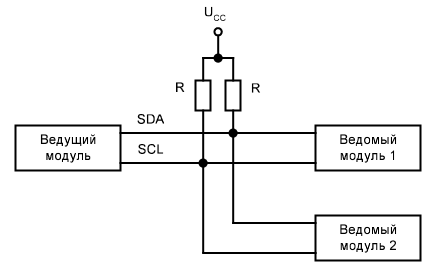
\includegraphics[width=0.525\textwidth]{../image/i2c.png}
    \caption{Организация интерфейса.}
	\end{figure}
	
	Интерфейс в микроконтроллере расположен на выводах PB10 (SCL) и PB11 (SDA). Также для дисплея потребуется питание 3.3 В.
	
	Дисплей и кнопки расположим на макетной плате размером 50 на 50 мм.
	
	\begin{figure}[H]
    \centering
    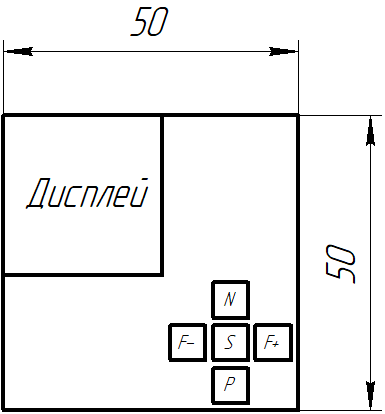
\includegraphics[width=0.45\textwidth]{../image/func_gen.png}
    \caption{Расположение периферии.}
	\end{figure}
	
	Назначения кнопок:
	\begin{enumerate}
	\item F- --- уменьшить частоту.
	\item F+ --- увеличить частоту.
	\item P --- предыдущий сигнал.
	\item N --- следующий сигнал.
	\item S --- переключить шаг по частоте.
	\end{enumerate}
	
	В результате сборки получилась плата с периферией.

	\begin{figure}[H]
    \centering
    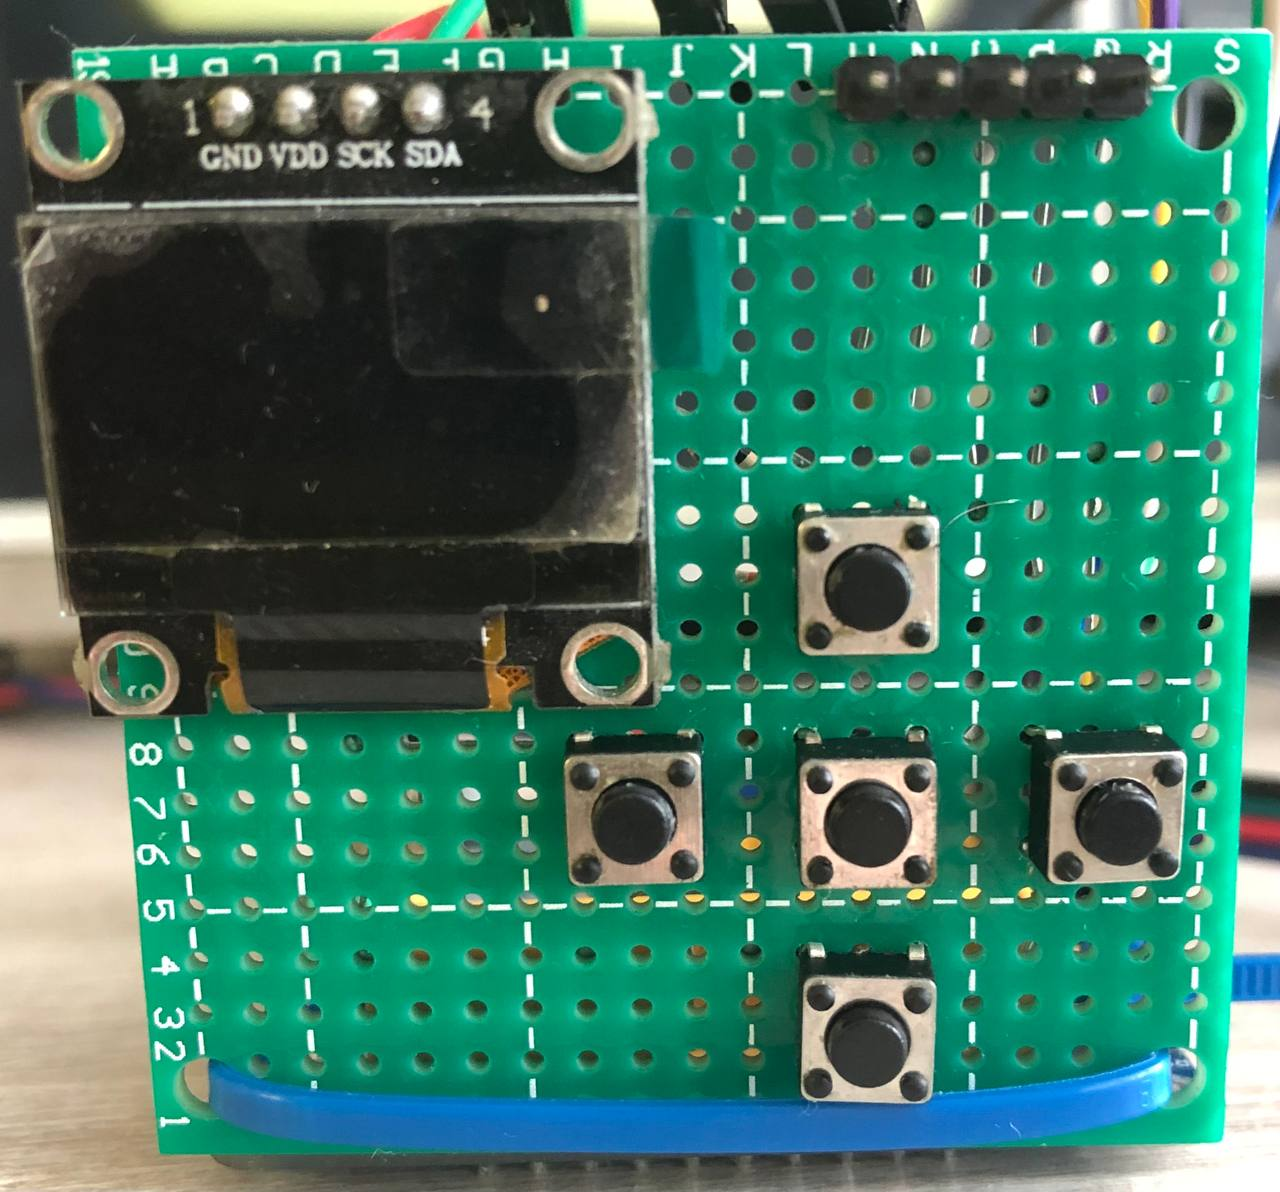
\includegraphics[width=0.65\textwidth]{../image/m1.jpeg}
    \caption{Плата периферии.}
	\end{figure}	
	
	Макет устройства будет состоять из отладочной платы микроконтроллера и полученной платы периферии. Обе части будут соединены проводами. Выход цифро-аналогового преобразователя, на котором генерируется сигнал, расположен на отладочной плате. В результате конструирования получился следующий макет устройства (рис. 3.6).

	\begin{figure}[H]
    \centering
    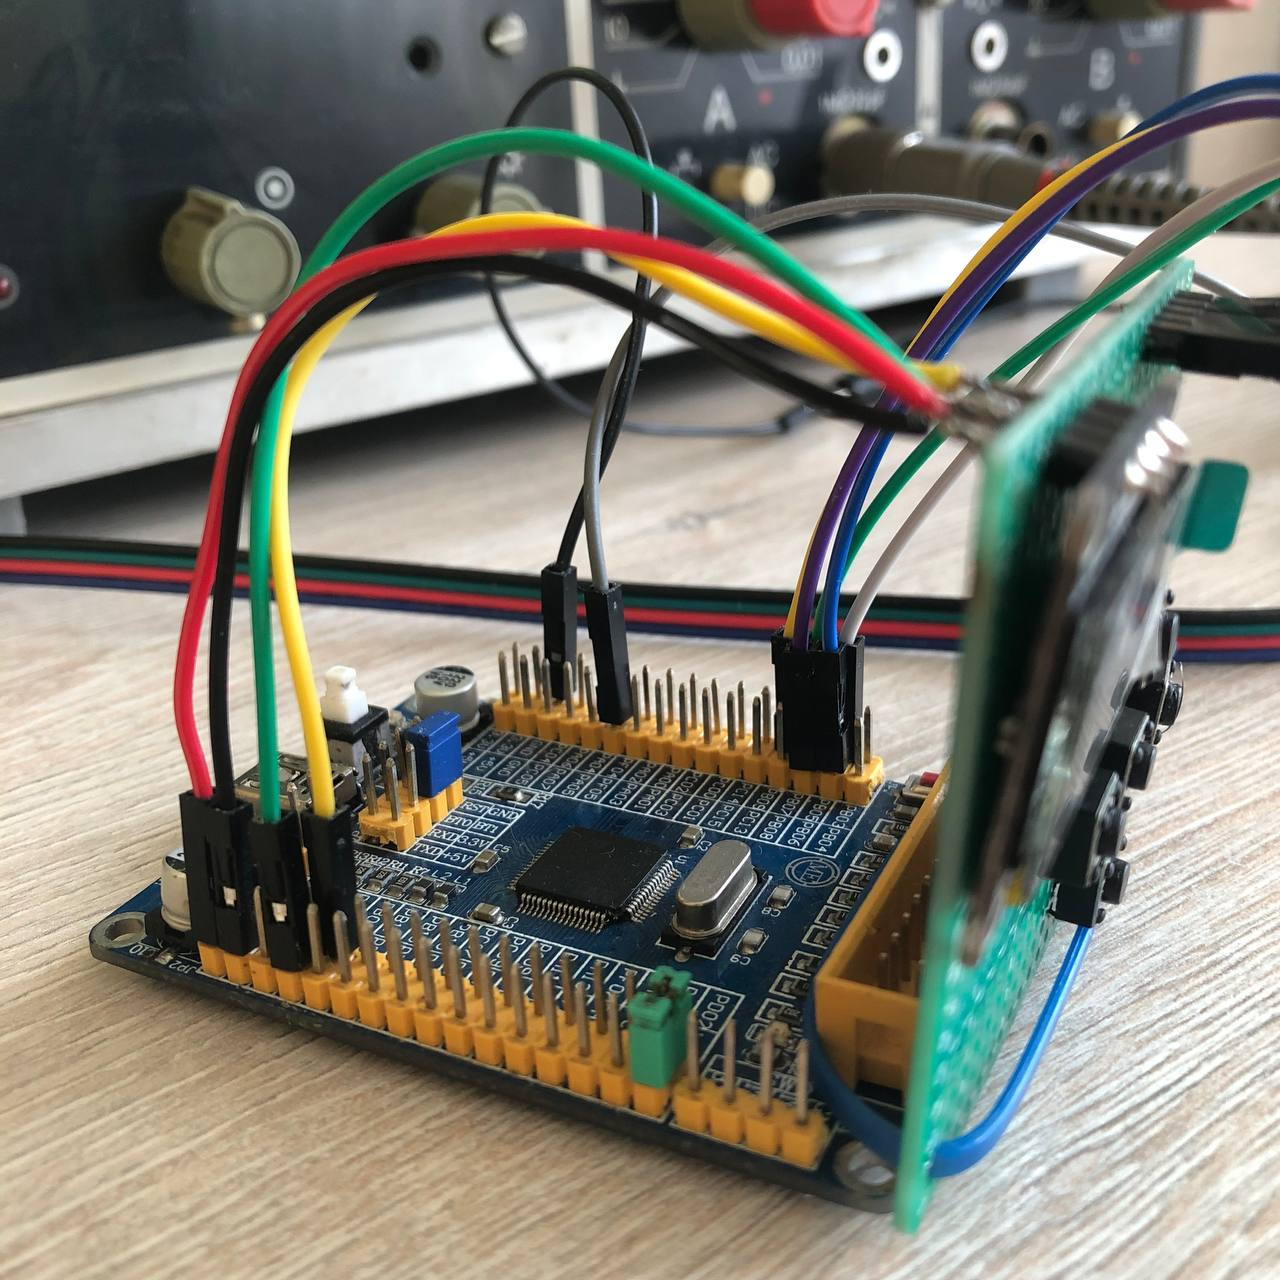
\includegraphics[width=0.65\textwidth]{../image/m2.jpeg}
    \caption{Макет устройства.}
	\end{figure}	

\section{Тестирование устройства}

\section{Вывод из третьей главы}